\documentclass[11pt,usenames,dvipsnames,svgnames,x11names]{beamer} 

\usetheme{Warsaw}
\usepackage{amssymb,amsmath,amsthm,amsfonts}                    
\usecolortheme{whale} 
\setbeamertemplate{navigation symbols}{}
\usepackage[utf8]{inputenc} 
\usepackage{polski}
\usepackage{tikz}
\usepackage{subfigure}
\usepackage{setspace}
\usepackage{savesym}
\savesymbol{arc}
\usepackage{color}
\usepackage{xcolor}
\usepackage{pict2e}
\usepackage{epstopdf}
\usepackage{caption}

\date{23 września 2013}
\author{Marta Sommer}
\title{Wymiar Hausdorffa zbioru granicznego IFS}

\theoremstyle{plain}
\newtheorem{twierdzenie}{Twierdzenie} 
\newtheorem{twierdzeniecd}{Twierdzenie cd.} 
\theoremstyle{definition}
\newtheorem{definicja}{Definicja}
\newtheorem{przyklad}{Przykład}
\newtheorem{lemat}{Lemat}
\newtheorem{wniosek}{Wniosek}
\newtheorem{oznaczenia}{Oznaczenia}
\theoremstyle{remark}
\newtheorem{uwaga}{Uwaga}

%\setbeamercovered{transparent}

\begin{document}


\begin{frame}   %tytułowa
\titlepage
\end{frame}

\begin{frame}   %ifs
\frametitle{IFS}
	\begin{definicja}
		Iterowanym układem funkcyjnym (IFS - \textit{iterated function system}) nazywamy rodzinę kontrakcji $\lbrace S_1,\ldots,S_m\rbrace$ taką, że $S_i:\hspace{1mm} D \longrightarrow D$, gdzie $D\subset\mathbb{R}^n$.
	\end{definicja}
\end{frame}

\begin{frame}   %trójkąt sierpińskiego + ifs
\frametitle{Trójkąt Sierpińskiego}

	\begin{center}
		\begin{figure}[htbp]
			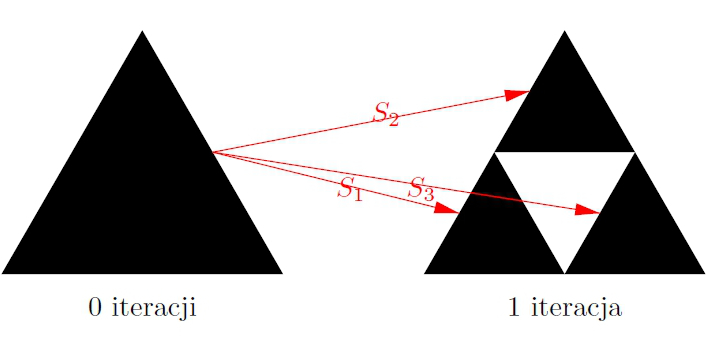
\includegraphics[scale=0.3]{bs1.jpg}
		\end{figure}
	\end{center}
$$
\aligned
S_1(x,y)&=\left(\frac{1}{2}x,\frac{1}{2}y\right),\\
S_2(x,y)&=\left(\frac{1}{2}x+\frac{1}{4},\frac{1}{2}y+\frac{\sqrt{3}}{4}\right),\\
S_3(x,y)&=\left(\frac{1}{2}x+\frac{1}{2},\frac{1}{2}y\right).
\endaligned
$$
\end{frame}

\begin{frame}   %tw o istnieniu atraktora
\frametitle{Twierdzenie o istnieniu atraktora}
\begin{twierdzenie}

Rozważmy IFS określony na zbiorze $D \subset \mathbb{R}^{n}$ kontrakcjami $ \lbrace S_1, \ldots,S_m \rbrace $. Wtedy istnieje jednoznacznie wyznaczony atraktor~$F$, tj. niepusty i zwarty zbiór taki, że:

$$
F = \bigcup^{m}_{i=1}{S_i(F)}. 
$$
\end{twierdzenie}
\end{frame}

\begin{frame}   % trójkąt sierpińskiego
\frametitle{Trójkąt Sierpińskiego}
\begin{center}
		\begin{figure}[htbp]
			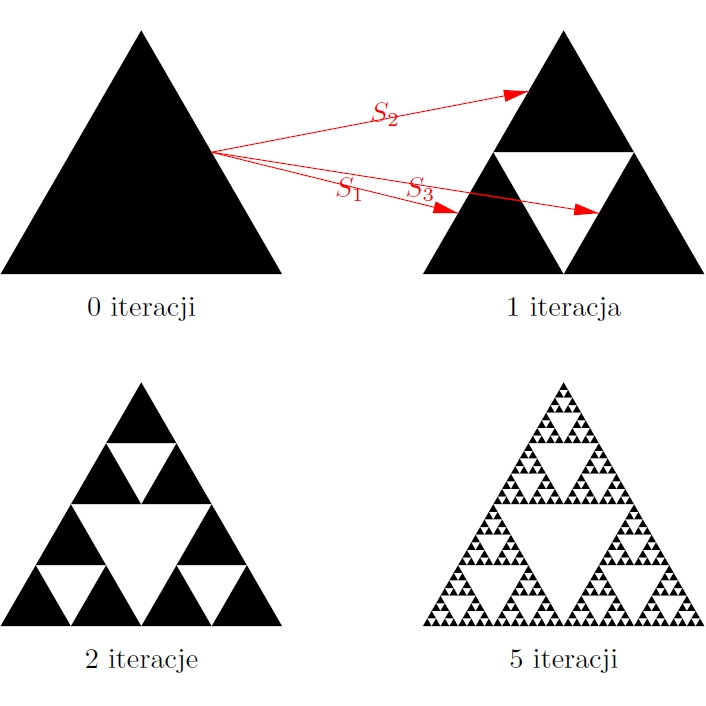
\includegraphics[scale=0.3]{bs.jpg}
		\end{figure}
	\end{center}
\end{frame}

\begin{frame}   %tw o istnieniu atraktora cd.
\frametitle{Twierdzenie o istnieniu atraktora cd.}
\begin{twierdzeniecd}

Zdefiniujmy dodatkowo przekształcenie $S$ na klasie $X$ niepustych i~zwartych podzbiorów~$D$ jako:

$$
\forall_{E \in X} \hspace{5mm} S(E) = \bigcup^{m}_{i=1} S_i(E)
$$

oraz oznaczymy przez $S^k$  $k$-tą iterację $S$ tzn. 

$$ 
\left\{ 
\begin{array}{l}
S^0(E) = E ,\\
S^k(E) = S\left(S^{k-1}(E)\right) \hspace{4mm}\textrm{dla} \hspace{2mm} k \geq 1, 
\end{array}
\right.
$$

wtedy:

$$
\forall_{E \in X \hspace{2mm} \textrm{takiego, że} \hspace{2mm} \forall_{i=1,\ldots ,m} \hspace{2mm} S_i(E) \subset E} \hspace{5mm} F = \bigcap^{\infty}_{k=0} S^k(E).
$$
\end{twierdzeniecd}
\end{frame}

\begin{frame}   %open set condition
\frametitle{Warunek zbioru otwartego}
\begin{definicja}
Funkcje $S_1,\ldots,S_m$ takie, że $S_i:D \longrightarrow D$, spełniają warunek zbioru otwartego (\textit{open set condition}), jeśli istnieje niepusty, ograniczony i otwarty zbiór $V$ taki, że:
$$
\bigcup^{m}_{i=1}S_i(V) \subset V
$$

oraz $S_i(V)$ są parami rozłączne dla $i=1,\ldots,m$. 
\end{definicja}
\end{frame}

\begin{frame}   %tw o wymiarze fraktali
\frametitle{Twierdzenie o wymiarze fraktali}
	\begin{twierdzenie}
Przypuśćmy, że podobieństwa $S_1,\ldots,S_m$ określone na $\mathbb{R}^n$ ze stałymi $c_i \in (0,1)$ dla $i=1,\ldots,m$, spełniają warunek zbioru otwartego.

Jeśli $F$ jest atraktorem IFS $\lbrace S_1,\ldots,S_m\rbrace$ tzn. 
$$
F = \bigcup^{m}_{i=1}{S_i(F)},
$$

wtedy $\dim_HF=s$, gdzie $s$ jest rozwiązaniem równania:

$$
\sum^m_{i=1}c_i^s=1.
$$

Co więcej, dla tej wartości $s$, $0<\mathcal{H}^s(F)<\infty$.
	\end{twierdzenie}
\end{frame}

\begin{frame}   %wymiar trójkąta sierpińskiego
\frametitle{Wymiar Hausdorffa trójkąta Sierpińskiego}

$$c_1=c_2=c_3=\frac{1}{2}$$

$$
\aligned
\sum_{i=1}^3 c_i^s&=1\\
c_1^s+c_2^s+c_3^s&=1\\
2^s&=3 \\
s&=\log_2 3 = 1.58496\ldots 
\endaligned
$$

Wymiar Hausdorffa trójkąta Sierpińskiego jest więc równy $\log_23 \approx 1.58$.

\end{frame}

\begin{frame}
\frametitle{Fraktal 1}
	\begin{center}
		\begin{figure}[htbp]
			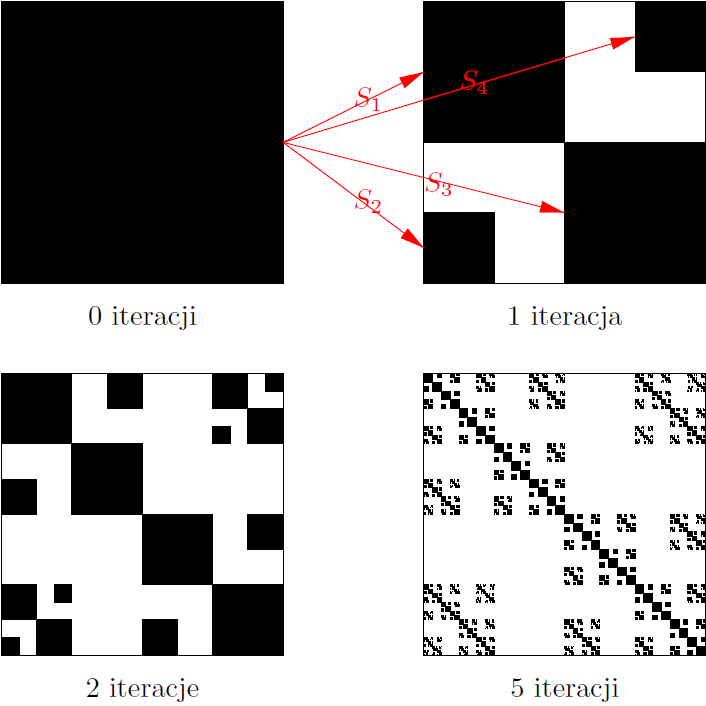
\includegraphics[scale=0.3]{serwetka.jpg}
		\end{figure}
	\end{center}
\end{frame}

\begin{frame}
\frametitle{Wymiar Hausdorffa atraktora}
$$c_1=c_3=\frac{1}{4},~c_2=c_4=\frac{1}{2}$$

$$
\aligned
\sum_{i=1}^4 c_i^s&=1\\
2\cdot \left(\frac{1}{4}\right)^s+2\cdot\left(\frac{1}{2}\right)^s&=1\\
s&=\log_2 \frac{2}{-1+\sqrt{3}}= 1.449984\ldots\\
\endaligned
$$

Wymiar Hausdorffa tak utworzonego fraktala jest więc równy $\log_2 \frac{2}{-1+\sqrt{3}}~\approx~1.45$.
\end{frame}

\begin{frame}
\frametitle{Fraktal 2}
	\begin{center}
		\begin{figure}[htbp]
			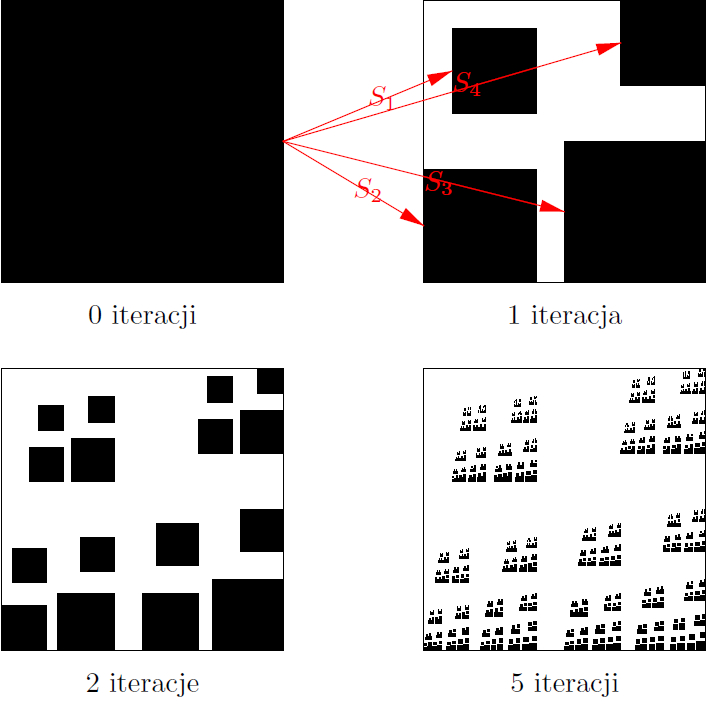
\includegraphics[scale=0.3]{kwadrat.jpg}
		\end{figure}
	\end{center}
\end{frame}

\begin{frame}
\frametitle{Wymiar Hausdorffa atraktora}
$$c_1=0.3,~c_2=0.4,~c_3=0.5,~c_4=0.3$$
$$
\aligned
\sum_{i=1}^4 c_i^s&=1\\
0.4^s+0.5^s+2\cdot0.3^s&=1\\
\endaligned
$$

Nie da się wyznaczyć $s$ analitycznie. Z numerycznej metody bisekcji otrzymujemy, że:
$$
s\simeq 1.428292002903.
$$
Wymiar Hausdorffa atraktora tego fraktala jest więc równy w przybliżeniu $1.43$.

\end{frame}

\begin{frame}   %dziękuję
\frametitle{~}
\begin{center}
\Large{Dziękuję za uwagę}
\end{center}

\end{frame}


\end{document}
